\section{Introduction}
Nowadays, a huge number of different products are produced worldwide. Thus, people have more options, leading producers to consider increasing their sales. Thus, they tried to determine each individual's personality and advertise the products customized to their personality type. 
Collecting such data is challenging for researchers because many people don't know their personality type. Thus, researchers tried to extract the personality of people from their tweets. There are other problems because they cannot determine people's personalities just by reading a tweet. Therefore, they are dependent on people again to determine their own personality.
With data generation, we hope to overcome these problems. I put my code for this project on my GitHub\footnote{https://github.com/Babakbehkamkia/Data-Generation-for-Personality-Detection}.



% \section{Word2vec}

% write the full name of dataset
\section{Language Model}
In this section, I have fine-tuned GPT2 by using Myers-Briggs Personality Type Dataset\footnote{https://www.kaggle.com/datasets/datasnaek/mbti-type/code} for each label. Then, I generated some samples and stored them in the stats folder. Here are some of the generated samples by fine-tuned GPT2: 
\begin{itemize}
    \item A nice way to start with when the people start calling and ask about my plans.
    \item Now, I just get weird looks :) and it usually doesn't get a bit of responses.
    \item And what's with guys saying they have one friend?! They must be totally lonely, it sounds more a woman thing with ENFJ too..
    \item This guy is actually my avatar's picture so i thought of it
    \item Do we not have some other similar stories like these we can share?  We have talked for hours over it
\end{itemize}



\section{Feature Engineering}

\begin{figure}[H]
    \centering
    \subfloat[accuracy]{%
        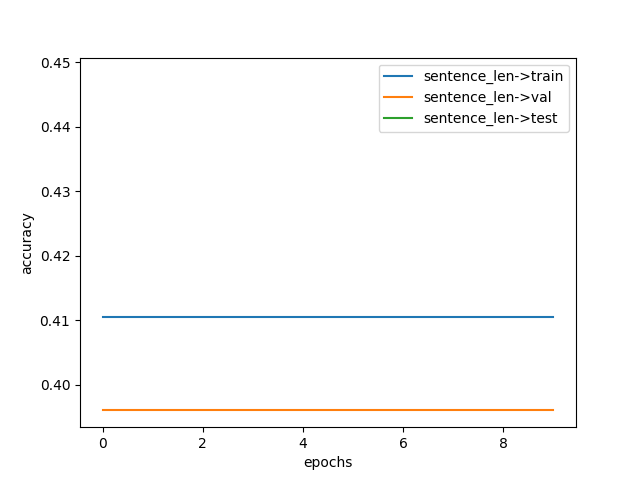
\includegraphics[width=0.4\linewidth,height=0.2\textheight]{../stats/acc_plot_sentence_len.png}%
        }%
    \subfloat[loss]{%
        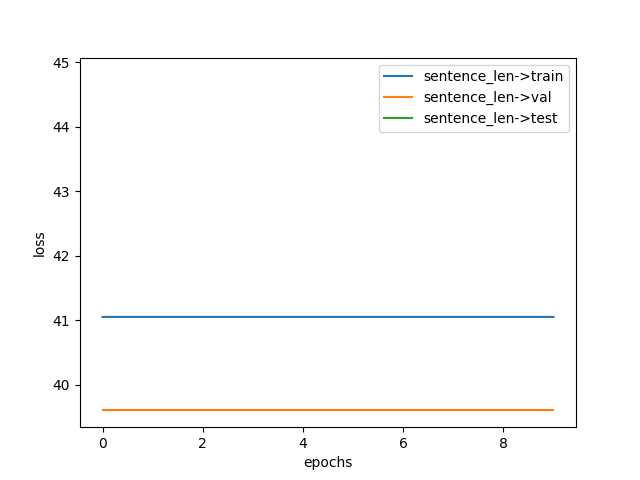
\includegraphics[width=0.4\linewidth,height=0.2\textheight]{../stats/loss_plot_sentence_len.png}%
        }%
\end{figure}


\begin{figure}[H]
    \centering
    \subfloat[accuracy]{%
        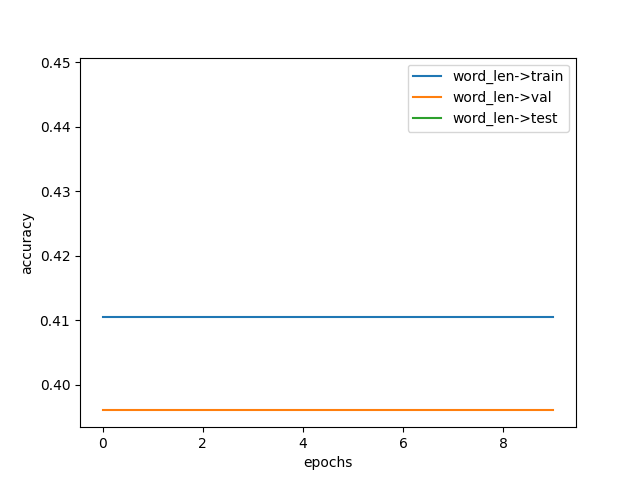
\includegraphics[width=0.4\linewidth,height=0.2\textheight]{../stats/acc_plot_word_len.png}%
        }%
    \subfloat[loss]{%
        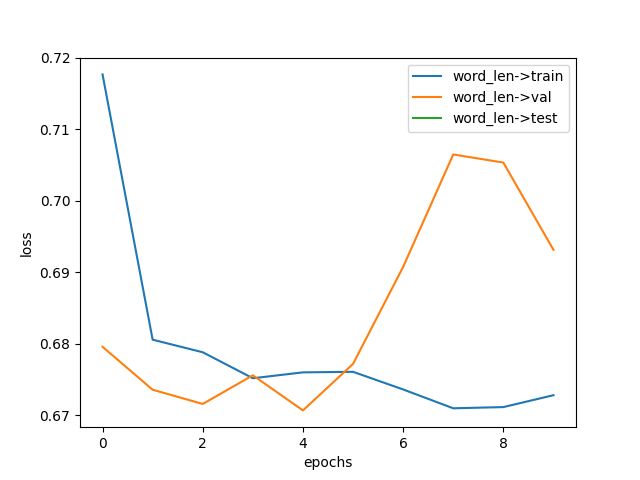
\includegraphics[width=0.4\linewidth,height=0.2\textheight]{../stats/loss_plot_word_len.png}%
        }%
\end{figure}


\begin{figure}[H]
    \centering
    \subfloat[accuracy]{%
        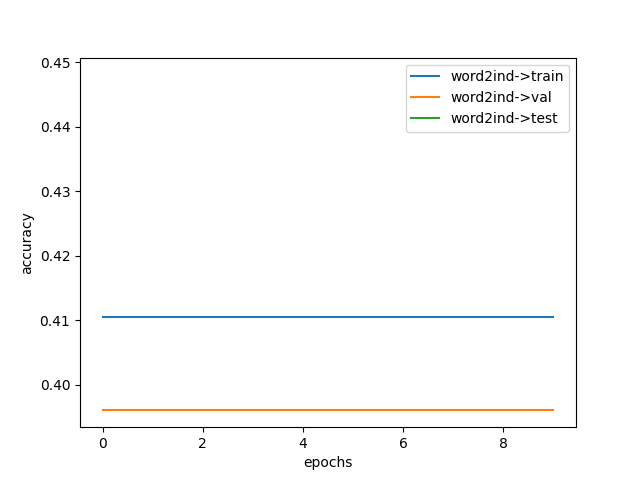
\includegraphics[width=0.4\linewidth,height=0.2\textheight]{../stats/acc_plot_word2ind.png}%
        }%
    \subfloat[loss]{%
        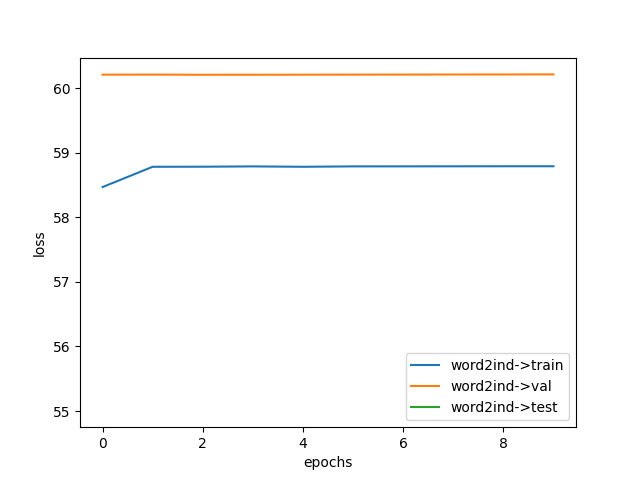
\includegraphics[width=0.4\linewidth,height=0.2\textheight]{../stats/loss_plot_word2ind.png}%
        }%
\end{figure}

\begin{figure}[H]
    \centering
    \subfloat[accuracy]{%
        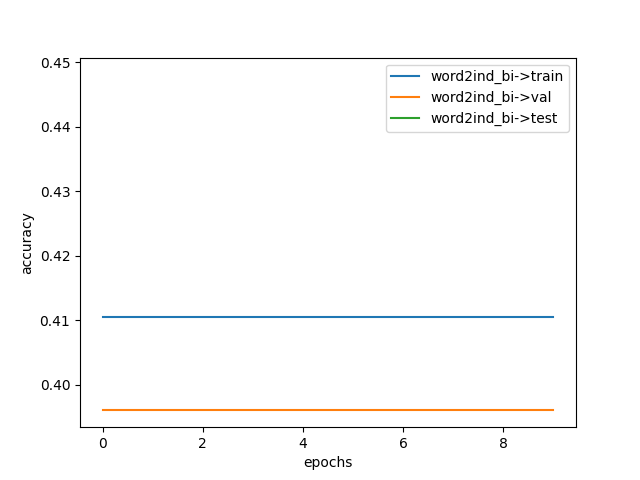
\includegraphics[width=0.4\linewidth,height=0.2\textheight]{../stats/acc_plot_word2ind_bi.png}%
        }%
    \subfloat[loss]{%
        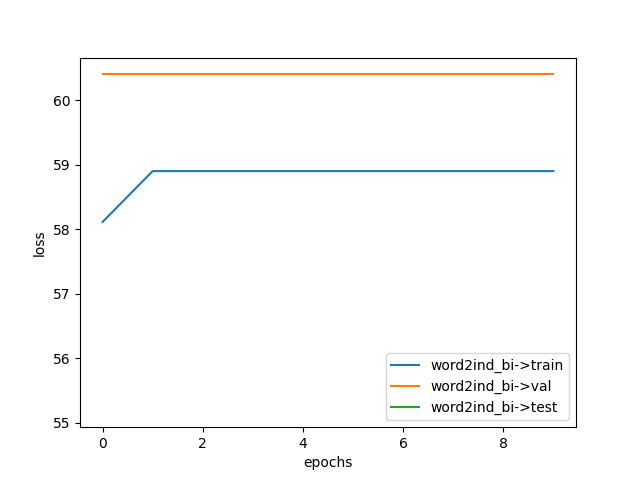
\includegraphics[width=0.4\linewidth,height=0.2\textheight]{../stats/loss_plot_word2ind_bi.png}%
        }%
\end{figure}


\begin{figure}[H]
    \centering
    \subfloat[accuracy]{%
        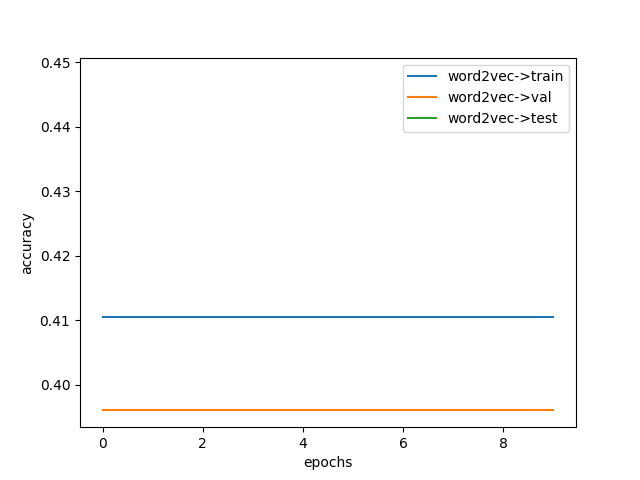
\includegraphics[width=0.4\linewidth,height=0.2\textheight]{../stats/acc_plot_word2vec.png}%
        }%
    \subfloat[loss]{%
        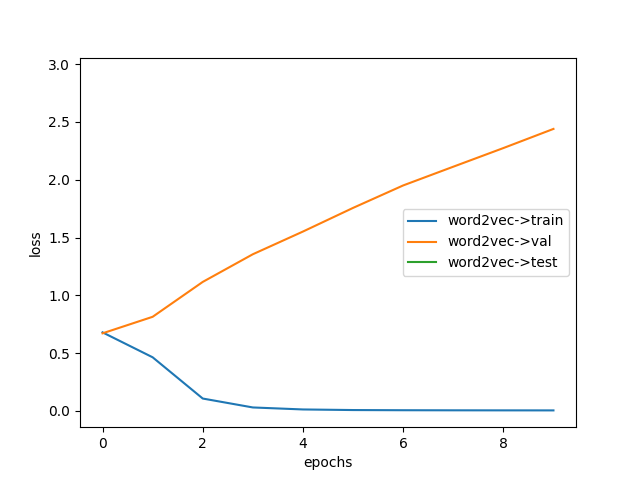
\includegraphics[width=0.4\linewidth,height=0.2\textheight]{../stats/loss_plot_word2vec.png}%
        }%
\end{figure}


\begin{figure}[H]
    \centering
    \subfloat[accuracy]{%
        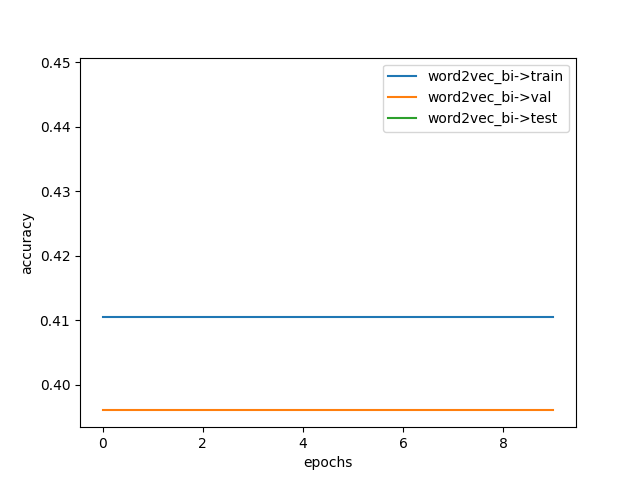
\includegraphics[width=0.4\linewidth,height=0.2\textheight]{../stats/acc_plot_word2vec_bi.png}%
        }%
    \subfloat[loss]{%
        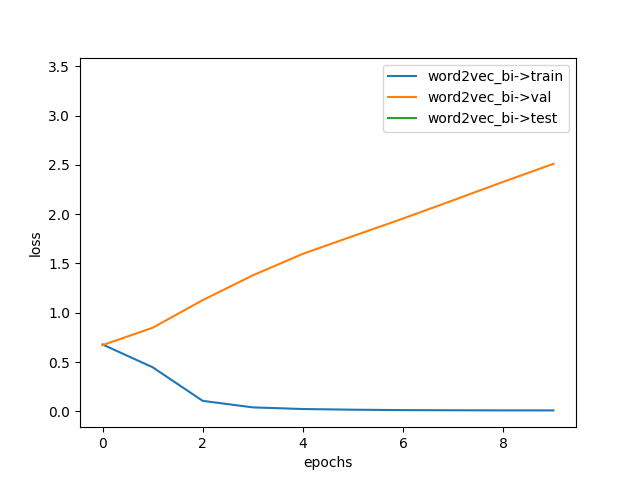
\includegraphics[width=0.4\linewidth,height=0.2\textheight]{../stats/loss_plot_word2vec_bi.png}%
        }%
\end{figure}


\begin{figure}[H]
    \centering
    \subfloat[accuracy]{%
        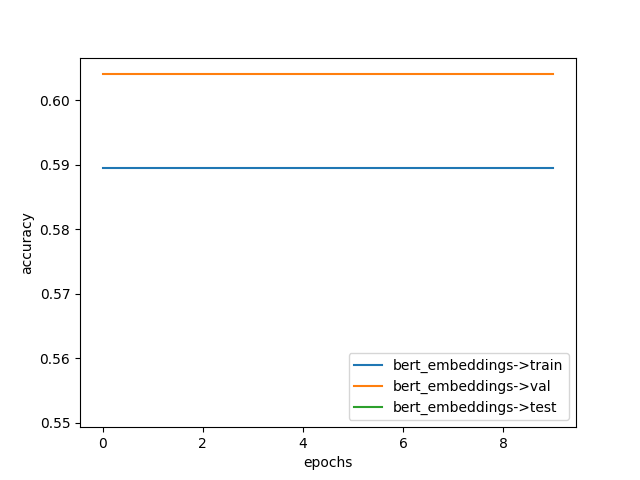
\includegraphics[width=0.4\linewidth,height=0.2\textheight]{../stats/acc_plot_bert_embeddings.png}%
        }%
    \subfloat[loss]{%
        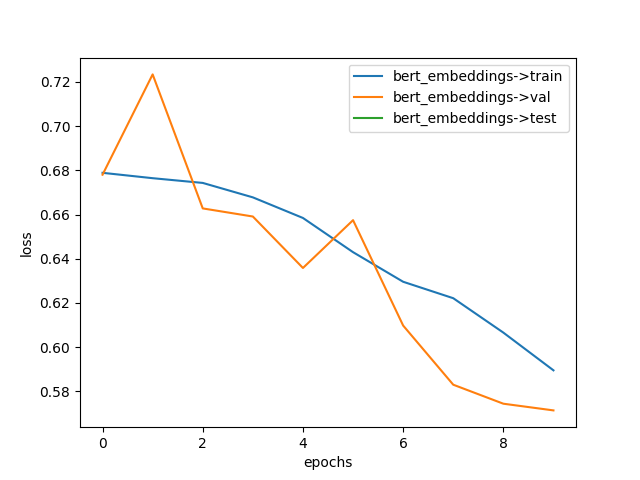
\includegraphics[width=0.4\linewidth,height=0.2\textheight]{../stats/loss_plot_bert_embeddings.png}%
        }%
\end{figure}


Although we used only two labels of the dataset, the results are bad because of many reasons. First, we used only one feature for each one which is not enough. Second, the used features are not suitable to train a deep learning model. Finaly, the structure of model is too simple.

\section{Model Architecture}
In this part, I used the end-to-end BERT model to predict the personalities. It gets 43\% accuracy. I also tried a convolutional layer on bert embeddings which does not lead to a good result.


\section{Data Augmentation}
I have generated some related data by using the GPT3 API in the previous phase. Here are some examples of generated data:


\begin{itemize}
    \item Love is a complex and intriguing concept . As an [PT] , I tend to analyze and dissect the different components of love , including attraction , chemistry , and compatibility . While I may seem guarded when it comes to matters of the heart , I value deep and meaningful connections with others
    \item Cinema offers a wealth of opportunities to explore different perspectives and thought-provoking ideas . As an [PT] , I enjoy movies that challenge my intellect and expand my understanding of the world around me . I tend to favor films with complex characters and intricate plotlines that keep me engaged and guessing until the very end
\end{itemize}


\section{OpenAI}
In this part, I have prepared a prompt in order to force GPT3 to do the personality detection. Here is the prompt I used for zero-shot learning:
 \\
\fbox{\begin{minipage}{12 cm}
Your task is to predict the possible personality of the writer of a text which is delimited by three backticks.


                There are four distinct classifications for this task.

                
                classification 1 classes: "Extrovert" and "Introvert"

                
                classification 1 labels: "E" and "I" respectively

                
                classification 2 classes: "Sensors" and "Intuitives" \\
                classification 2 labels: "S" and "N" respectively \\
                classification 3 classes: "Thinkers" and "Feelers" \\
                classification 3 labels: "T" and "F" respectively \\
                classification 4 classes: "Judgers" and "Perceivers" \\
                classification 4 labels: "J" and "P" respectively \\
                only give the predicted label for each classification. It means that you need to give 4 answers. Concatinate the labels with eachother in the above order. \\
                give only one answer for each classification. be carful about the order of your answer, it is important. \\
                For example this could be two sample answers (learn the format of the output, do not copy): \\
                sample answer1: \\
                  "ENTJ" \\
                sample answer2: \\
                  "INFJ" \\

                text: ```{text}```
\end{minipage}}


The accuracy for a small proportion of our data (about 1\%) was 4\%. I used the same prompt for the few-shot learning with two additional tweets and their labels. The accuracy for the few-shot was 5\%.
\\
\\
\textbf{Note:} Due to our limited access to GPT3 API, I used only 10 tweets out of 50 for each sample. Moreover, I assume this task is a 16-class classification and an answer considered a true prediction when it predicts all four traits correctly.

% \section{Scripts}
% For this work, bash and batch scripts are provided to run each part or the entire project. The necessary instructions are inside those files.